\documentclass[a4paper,11pt,oneside]{article}
\usepackage[ngerman]{babel} % für die deutsche Sprache
\usepackage[T1]{fontenc} % Schriftkodierung (Für Sonderzeichen u.a.)
\usepackage[utf8]{inputenc} % Für die direkte Eingabe von Umlauten im Editor u.a.
\usepackage{fancyhdr} % Für Kopf- und Fußzeilen
\usepackage{lmodern} % Schriftart "Latin Modern"
%\usepackage[normalem]{ulem} % Für das Unterstreichen von Text z.B. mit \uline{}
\usepackage[left=2cm,right=3cm,top=1cm,bottom=1cm,
textheight=245mm,textwidth=160mm,includeheadfoot,headsep=1cm,
footskip=1cm,headheight=14.599pt]{geometry} % Einrichtung der Seite 
\usepackage{setspace} % Paket zum Setzen des Zeilenabstandes
\usepackage{graphicx} % Zum Laden von Graphiken
\usepackage{amsmath}
\usepackage{amsthm}
\usepackage{amsfonts}
\usepackage{hyperref} % Hyperlinks im Inhaltsverzeichnis
\usepackage{pdfpages}
\usepackage{csquotes}
\usepackage{float}

\title{Kurzanleitung zum Erstellen von PLECS-Simulationsskripten}
\author{Jonathan Koeppen}
\date{\today}

\usepackage[style=numeric,sorting=none]{biblatex} % Stil hier angeben
\addbibresource{Literatur.bib} % .bib Datei hier einbinden

\onehalfspacing

\begin{document}
	\maketitle
	\newpage
	\pagestyle{fancy}
	\tableofcontents
	\setcounter{section}{1}
	\section*{PLECS Analysis Tool}
Die PLECS Analyse-Tools können zur Durchführung von stationären und Kleinsignalanalysen verwendet werden. Mit dem Tool zur stationären Analyse kann der stationäre Arbeitspunkt des Systems gefunden werden, und die Kleinsignalanalyse-Tools können offene und geschlossene Übertragungsfunktionen ermitteln. Es stehen drei Arten von Kleinsignalanalysen zur Verfügung: AC Sweep, Impulsantwortanalyse und Multitonanalyse.

Dieser Abschnitt konzentriert sich auf die Anwendung dieser Tools in der Systemsimulation.
Als fortführendes Dokument wird das Dokument analysis\_tool.pdf empfohlen, welches im Ordner dieses Dokuments abgelegt ist oder unter \href{https://www.plexim.com/sites/default/files/tutorials_categorized/plecs/analysis_tools.pdf}{diesem Link} zu finden ist.

\subsection{Werkzeugübersicht}
PLECS Standalone bietet spezielle stationäre und Kleinsignalanalyse-Tools, die über das Menü Simulation $\rightarrow$ Analyse-Tools... zugänglich sind.
\subsection{Stationäre Analyse}
Die meisten dynamischen Systeme durchlaufen einen anfänglichen dynamischen Transientenprozess und erreichen schließlich einen stationären Zustand. Der stationäre Zustand eines Systems wird erreicht, wenn alle Zustandsvariablen entweder nicht mehr ändern (DC-Arbeitspunkt) oder sich periodisch ändern (periodischer Arbeitspunkt).

\begin{figure}[h]
	\centering
	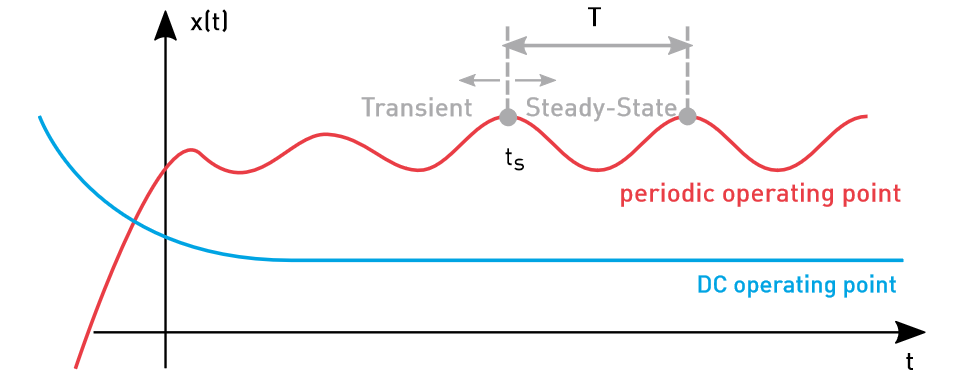
\includegraphics[width=0.8\textwidth]{steady_state.png}
	\caption{Periodische und DC-Arbeitspunkte}
\end{figure}

\textbf{Wichtige Anforderungen:}
\begin{itemize}
	\item Die Systemperiode $T$ ist das kleinste gemeinsame Vielfache der Perioden aller Wechselstromquellen im System. Wenn 'auto' ausgewählt ist, versucht PLECS, diese Zahl zu berechnen. Bei speziellen Blöcken, deren Implementierung PLECS unbekannt ist, muss die Systemperiode vom Benutzer berechnet werden.
	\item Die Systemperiode $T$ muss vor der Analyse bekannt sein und im Parameterfeld 'Systemperiode' angegeben werden.
	\item Es dürfen während der Analyse keine Transienten im System auftreten, außer bei periodischen Quellen.
\end{itemize}

\textbf{Wichtige Parameter:}
\begin{itemize}
	\item Arbeitspunkt: Definiert, ob das System periodisch oder nicht periodisch (DC) ist.
	\item Systemperiode: Das kleinste gemeinsame Vielfache der Perioden aller Wechselstromquellen im System.
	\item Simulationsstartzeit: Die Startzeit für die Transientsimulationen.
	\item Anzahl der finalen Zyklen / Zeitspanne: Anzahl der stationären Zyklen, die am Ende der Analyse angezeigt werden.
	\item Anzahl der Initialisierungszyklen: Anzahl der zyklusweisen Simulationen vor Beginn der Newton-Iterationen.
	\item Abbruchtoleranz: Relative Fehlergrenze für die Konvergenz.
	\item Maximale Anzahl von Iterationen: Maximale erlaubte Iterationen.
	\item Relative Perturbation für Jacobian: Relative Perturbation zur Berechnung der Jacobian-Matrix.
	\item Jacobian-Berechnung: Methode zur Berechnung der Jacobian-Matrix-Einträge (vollständig oder schnell).
	\item Maximale Anzahl von Threads: Maximale erlaubte parallele Threads.
\end{itemize}

\subsection{Kleinsignalanalyse}
Die Kleinsignalanalyse-Tools helfen bei der Reglerauslegung, indem sie die Übertragungsfunktion des Systems berechnen und die Stabilität des geschlossenen Regelkreises vorhersagen.

Die verfügbaren Kleinsignalanalysen sind:
\begin{itemize}
	\item AC Sweep: Verwendet sinusförmige Perturbationen, um die Systemantwort bei verschiedenen Frequenzen zu analysieren.
	\item Impulsantwortanalyse: Verwendet einen einzelnen Impuls, um das System zu perturbieren und berechnet die Übertragungsfunktion aus der Laplace-Transformation der transienten Antwort.
	\item Multitonanalyse: Verwendet ein Multiton-Signal, das aus mehreren Sinussignalen besteht, um die Systemantwort zu analysieren.
\end{itemize}

Wichtige Parameter für Kleinsignalanalysen:
\begin{itemize}
	\item Arbeitspunkt: Definiert, ob das System periodisch oder nicht periodisch (DC) ist.
	\item Systemperiode: Das kleinste gemeinsame Vielfache der Perioden aller Quellen.
	\item Frequenzbereich: Bereich der Perturbationsfrequenzen.
	\item Amplitude: Amplitude des Perturbationssignals.
	\item Perturbation: Der während der Analyse aktive Small Signal Perturbation Block.
	\item Antwort: Der Small Signal Response Block, der die Systemantwort aufzeichnet.
	\item Simulationsstartzeit: Startzeit für die Transientsimulationen.
	\item Frequenzskala: Lineare oder logarithmische Verteilung der Sweep-Frequenzen.
	\item Anzahl der Punkte: Anzahl der automatisch verteilten Frequenzen.
	\item Zusätzliche Frequenzen: Zusätzliche zu sweepende Frequenzen.
	\item Maximale Anzahl von Threads: Maximale erlaubte parallele Threads.
\end{itemize}	
	
	\subsubsection{Verwendung im Regelentwurf}
	\textbf{Übertragungsfunktion der Regelgröße zum Ausgang:}
	Der erste Schritt im Entwurfsprozess besteht darin, die Übertragungsfunktion des Systems zu finden. Diese beschreibt, wie stark und wie schnell sich der Ausgang als Reaktion auf Änderungen des Eingangs ändert.
	
	\begin{figure}[H]
		\centering
		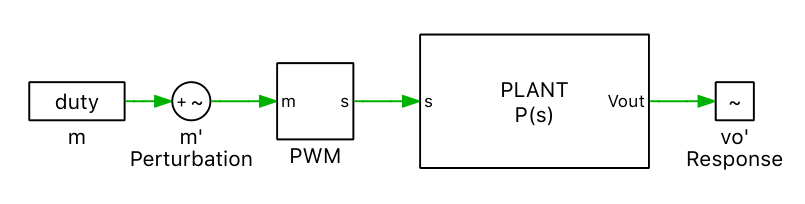
\includegraphics[width=0.8\textwidth]{open_loop.png}
		\caption{System mit offenem Regelkreis (open loop)}
	\end{figure}
	
	Die Übertragungsfunktion des Systems in Abbildung 2 ist:
	\[ P(s) = \frac{V_o(s)}{m(s)} \]
	
	Komponenten der Kleinsignalanalyse aus der PLECS Control Bibliothek werden verwendet, um diese Übertragungsfunktion zu erhalten. Der "Small Signal Perturbation"-Block erzeugt (oder injiziert) das geeignete Störsignal und der "Small Signal Response"-Block misst die Systemantwort für die Kleinsignalanalyse.
	
	\textbf{Offene Schleifenverstärkung / open loop gain :}
	Nach dem Entwurf des Reglers basierend auf der Übertragungsfunktion kann die Stabilität des geschlossenen Regelkreises durch Berechnung der offenen Schleifenverstärkung vorhergesagt werden.
	Der „Small Signal Gain“ (oder Loop Gain Meter) Block, wie in Abb. 3 gezeigt, misst die offene Schleifenverstärkung eines geschlossenen Regelkreises. Dieser Block verwendet zunächst den „Small Signal Perturbation“ Block, um eine Störung in eine Rückkopplungsschleife einzuspeisen, und dann den „Small Signal Response“ Block, um die Systemantwort zu messen. Dies ermöglicht es der „Loop Gain Meter“ Komponente, die Rückkopplungsschleife zu unterbrechen, während die Werte des Rückkopplungsausgangs weiterhin aktualisiert werden, um die Schleifenverstärkung zu berechnen. Die gemessene offene Schleifenverstärkung des geschlossenen Regelkreissystems ist $C(s)*P(s)$.
	\begin{figure}[H]
		\centering
		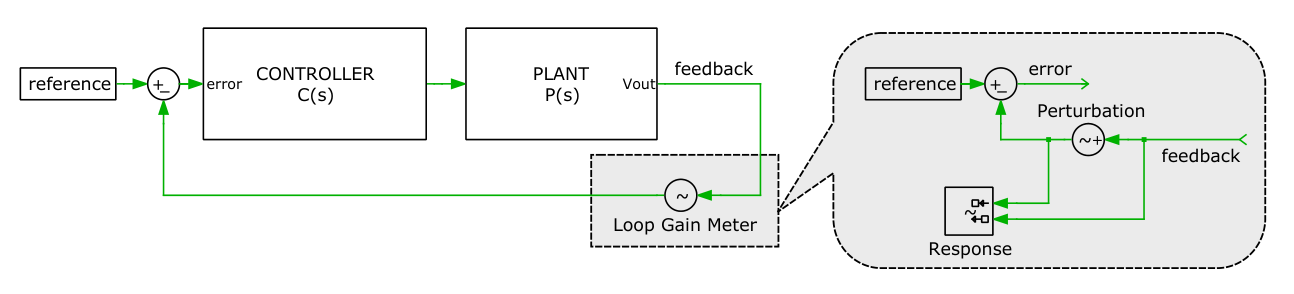
\includegraphics[width=0.8\textwidth]{closed_loop.png}
		\caption{System mit geschlossenem Regelkreis (closed loop)}
	\end{figure}
	
	\subsection{Übersicht über die verschiedenen Arten der Kleinsignalanalyse:}
	
	\begin{table}[H]
		\centering
		\resizebox{\textwidth}{!}{%
			\begin{tabular}{|l|c|c|c|c|}
				\hline
				Tool & \# Simulationen pro Analyse & Loop Gain Berechnung & Stationäre Analyse & Typ des stationären Zustands \\ \hline
				Multiton & 2 & Ja & Transient & Periodisch \& DC \\ \hline
				AC Sweep & n & Ja & Iterativ & Periodisch \& DC \\ \hline
				Impulsantwort & 1 & Nein & Iterativ & Periodisch \\ \hline
			\end{tabular}%
		}
		\caption{Übersicht der Analyse-Tools}
	\end{table}
	
	\textbf{Hauptschlussfolgerungen:}
	\begin{itemize}
		\item \# Simulationen pro Analyse: Eine Frequenzantwort besteht aus n einzelnen Frequenzen. Je nach Art der Perturbation (sinusförmig, Dirac-Impuls usw.) werden unterschiedliche Anzahlen von Simulationen benötigt.
		\item Loop Gain Berechnung: Die Impulsantwortanalyse unterstützt keine Loop Gain Berechnung.
		\item Stationäre Analyse: Nur die Multitonanalyse verwendet eine "brute force" Transientanalyse, um stationäre Bedingungen zu erreichen.
	\end{itemize}






	\newpage
	\printbibliography
\end{document}